\documentclass{article}
\usepackage[utf8]{inputenc}
% are all of these packages really necessary?
% no.
% i'm just too lazy to only grab the packages i want for a specific
% document, so i just glob all of my most commonly used packages together
% this is bad practice.
\usepackage{amsmath,amsthm,amssymb,amsfonts, fancyhdr, color, comment, graphicx, environ, mdframed, soul, calc, enumitem, mdframed, xcolor, geometry, empheq, mathtools, tikz, pgfplots, caption, subcaption, hyperref}

\usetikzlibrary{external}
\tikzexternalize[prefix=tikz/,optimize command away=\includepdf]

%tikzpicture
\usepackage{tikz}
\usepackage{scalerel}
\usepackage{pict2e}
\usepackage{tkz-euclide}
\usetikzlibrary{calc}
\usetikzlibrary{patterns,arrows.meta}
\usetikzlibrary{shadows}
\usetikzlibrary{external}
\usepackage{circuitikz}

%pgfplots
\usepackage{pgfplots}
\pgfplotsset{compat=newest}
\usepgfplotslibrary{statistics}
\usepgfplotslibrary{fillbetween}
\usepgfplotslibrary{polar}

\tikzset{external/export=true}
\pgfplotsset{
    standard/.style={
    axis line style = thick,
    trig format=rad,
    enlargelimits,
    axis x line=middle,
    axis y line=middle,
    enlarge x limits=0.15,
    enlarge y limits=0.15,
    every axis x label/.style={at={(current axis.right of origin)},anchor=north west},
    every axis y label/.style={at={(current axis.above origin)},anchor=south east}
    }
}
\newcommand*\widefbox[1]{\fbox{\hspace{2em}#1\hspace{2em}}}
% Command "alignedbox{}{}" for a box within an align environment
% Source: http://www.latex-community.org/forum/viewtopic.php?f=46&t=8144
\newlength\dlf  % Define a new measure, dlf
\newcommand\alignedbox[2]{
% Argument #1 = before & if there were no box (lhs)
% Argument #2 = after & if there were no box (rhs)
&  % Alignment sign of the line
{
\settowidth\dlf{$\displaystyle #1$}  
    % The width of \dlf is the width of the lhs, with a displaystyle font
\addtolength\dlf{\fboxsep+\fboxrule}  
    % Add to it the distance to the box, and the width of the line of the box
\hspace{-\dlf}  
    % Move everything dlf units to the left, so that & #1 #2 is aligned under #1 & #2
\boxed{#1 #2}
    % Put a box around lhs and rhs
}
}

\hypersetup{
    colorlinks=true,
    linkcolor=blue,
    filecolor=magenta,      
    urlcolor=cyan,
    pdftitle={Homework 20 Solutions},
    pdfpagemode=UseOutlines,
    bookmarksopen=true,
    pdfauthor={Christina Phan}
}
\newcommand{\lrp}[1]{\left( #1 \right)}
\newcommand{\abs}[1]{\left\vert #1 \right\vert}
\newcommand{\lra}[1]{\left\langle #1 \right\rangle}
\newcommand{\lrb}[1]{\left[ #1 \right]}
\newcommand{\norm}[1]{\left\lVert #1 \right\rVert}
\newcommand{\iintR}[0]{\iint\limits_{R}}
\renewcommand{\u}[0]{\mathbf{u}}
\renewcommand{\i}[0]{\mathbf{i}}
\renewcommand{\j}[0]{\mathbf{j}}
\renewcommand{\k}[0]{\mathbf{k}}
\newcommand{\T}[0]{\mathbf{T}}
\newcommand{\N}[0]{\mathbf{N}}
\newcommand{\B}[0]{\mathbf{B}}
\renewcommand{\r}[0]{\mathbf{r}}
\renewcommand{\a}[0]{\mathbf{a}}
\renewcommand{\v}[0]{\mathbf{v}}
\newcommand{\F}[0]{\mathbf{F}}
\newcommand{\n}[0]{\mathbf{n}}

\renewcommand{\arraystretch}{1.25}

\geometry{letterpaper, portrait, margin=1in}
\renewcommand{\footrulewidth}{0.8pt}
\setlength\parindent{0pt}
\pagestyle{fancy}
\lhead{Christina Phan}
\rhead{MAT 21D} 
\chead{\textbf{Homework 20 Solutions}}

\newcommand{\Solution}{\textit{Solution}}
\pgfplotsset{compat=1.18}
\begin{document}

\phantomsection
\addcontentsline{toc}{section}{Problem 1}\textbf{Problem 1}

Use a parametrization to evaluate $\displaystyle \iint_S \F\cdot \n\,d\sigma$ across the surface:

\phantomsection
\addcontentsline{toc}{subsection}{1(a)}\textbf{(a)} $\F(x,y,z)=\lra{0,x^2,-xz}$ outward (away from the $yz$-plane) through the surface cut from the parabolic cylinder $y=x^2$, $-1\leq x\leq 1$, by $z=0$ and $z=2$

\Solution

Since $y=x^2$, let's parameterize our cylinder as $\r(x,z)=\lra{x,x^2,z}$ where $-1\leq x\leq 1$ and $0\leq z\leq 2$.

Recall that if $S$ is given by the parameterization $\r(u,v)=\lra{x,y,z}$, then
\begin{align*}
    \iint_S \F\cdot \n \,d\sigma &= \iint_R \F \cdot \lrp{\frac{\partial \r}{\partial u}\times \frac{\partial \r}{\partial v}}\,dA
\end{align*}
In this problem, let's have our $u$ be $x$ and our $v$ be $z$.

Since $\r(x,z)=\lra{x,x^2,z}$,
\begin{align*}
\F&=\lra{0,x^2,-xz}\\
    \frac{\partial \r}{\partial x}&=\lra{1,2x,0}\\
    \frac{\partial \r}{\partial z}&=\lra{0,0,1}\\
    \frac{\partial \r}{\partial x}\times \frac{\partial \r}{\partial z}&=\begin{vmatrix}\i & \j & \k \\ 1 & 2x & 0\\ 0 & 0 & 1\end{vmatrix}\\
    &=\lrp{2x-0}\i - \lrp{1 - 0}\j + \lrp{0 - 0}\k\\
    &=\lrp{2x}\i - \lrp{1}\j + \lrp{0}\k\\
    &=\lra{2x,-1,0}
\end{align*}
Let's check if $\displaystyle  \frac{\partial \r}{\partial x}\times \frac{\partial \r}{\partial z}$ is in the right direction.

For no particular reason, at $x=1$ and $z=0$, we get the point $(1,1,0)$ from our parameterization. When $x=1$ and $z=0$, $\displaystyle\frac{\partial \r}{\partial x}\times \frac{\partial \r}{\partial z}=\lra{2,-1,0}$. Since $\lra{2,-1,0}$ at $(1,1,0)$ points away from the $yz$-plane, our direction for $\displaystyle  \frac{\partial \r}{\partial x}\times \frac{\partial \r}{\partial z}$ is correct.
\begin{center}
\resizebox{5cm}{!}{
    \begin{tikzpicture}
    \begin{axis}[standard,
            xtick={1,2,3},
            ytick={1,2,3},
            samples=1000,
            xlabel={$x$},
            ylabel={$y$ aka $yz$ plane},
            xmin=-.3,xmax=3.3,
            ymin=-.3,ymax=3.3,
            x=1cm,
            y=1cm/1,
           ]
\node[anchor=center,label=south west:$O$] at (axis cs:0,0){};
\draw (1,1) -- (3,0) node[
    currarrow,
    pos=1, 
    xscale=1,
    sloped,
    scale=1] {};
    \end{axis}
    \end{tikzpicture}
}
\end{center}

Since $\displaystyle  \frac{\partial \r}{\partial x}\times \frac{\partial \r}{\partial z}=\lra{2x,-1,0}$,
\begin{align*}
    \F \cdot \lrp{ \frac{\partial \r}{\partial x}\times \frac{\partial \r}{\partial z}}&=\lra{0,x^2,-xz}\cdot \lra{2x,-1,0}\\
    &=0-x^2-0\\
    &=-x^2
\end{align*}
Let's evaluate our integral.
\begin{align*}
    \iint_S \F\cdot \n \,d\sigma &=\int_{-1}^1\int_0^2 -x^2\,dz\,dx\\
    &=\int_{-1}^1\lrb{-x^2z}_0^2\,dx\\
    &=\int_{-1}^1 -2x^2\,dx\\
    &=\lrb{-\frac{2}{3}x^3}_{-1}^1\\
    &=\Big(-\frac{2}{3}(1)^3\Big)-\Big(-\frac{2}{3}\lrp{-1}^3\Big)\\
    &=\lrp{-\frac{2}{3}}-\lrp{\frac{2}{3}}\\
    &=\boxed{-\frac{4}{3}}
\end{align*}

\newpage
\phantomsection
\addcontentsline{toc}{subsection}{1(b)}\textbf{(b)} $\F(x,y,z)=\lra{x,y,z}$ across the sphere $x^2+y^2+z^2=a^2$ away from the origin

\Solution

Since we have a sphere of radius $a$, let's parameterize our sphere surface using spherical coordinates where $\rho = a$. That is, let $\r(\phi,\theta)=\lra{a,\sin\phi\cos\theta, a\sin\phi\sin\theta, a\cos\phi}$ where $0\leq \phi \leq \pi$ and $0\leq \theta\leq 2\pi$ since we're going around the entire sphere.


Recall that if $S$ is given by the parameterization $\r(u,v)=\lra{x,y,z}$, then
\begin{align*}
    \iint_S \F\cdot \n \,d\sigma &= \iint_R \F \cdot \lrp{\frac{\partial \r}{\partial u}\cdot \frac{\partial \r}{\partial v}}\,dA
\end{align*}
In this problem, let's have our $u$ be $\phi$ and our $v$ be $\theta$.

Since $\r(\phi,\theta)=\lra{a\sin\phi\cos\theta, a\sin\phi\sin\theta, a\cos\phi}$,
\begin{align*}
\F&=\lra{a\sin\phi\cos\theta, a\sin\phi\sin\theta, a\cos\phi}\\
    \frac{\partial \r}{\partial \phi}&=\lra{a\cos\phi\cos\theta, a\cos\phi\sin\theta, -a\sin\phi}\\
    \frac{\partial \r }{\partial \theta}&=\lra{-a\sin\phi\sin\theta, a\sin\phi\cos\theta, 0}\\
    \frac{\partial \r}{\partial \phi}\times  \frac{\partial \r }{\partial \theta}&=\begin{vmatrix}\i & \j & \k \\ a\cos\phi\cos\theta & a\cos\phi\sin\theta & -a\sin\phi \\ -a\sin\phi\sin\theta & a\sin\phi\cos\theta & 0\end{vmatrix}\\
    &=\lrp{0+a^2\sin^2\phi\cos\theta}\i-\lrp{0-a^2\sin^2\phi\sin\theta}\j +\lrp{a^2\sin\phi\cos\phi\cos^2\theta+a^2\sin\phi\cos\phi\sin^2\theta}\k\\
    &=\lrp{a^2\sin^2\phi\cos\theta}\i-\lrp{-a^2\sin^2\phi\sin\theta}\j + \big(a^2\sin\phi\cos\phi\lrp{\cos^2\theta+\sin^2\theta}\big)\k\\
    &=\lrp{a^2\sin^2\phi\cos\theta}\i-\lrp{-a^2\sin^2\phi\sin\theta}\j +\lrp{a^2\sin\phi\cos\phi}\k\tag{$\cos^2\theta+\sin^2\theta=1$}\\
    &=\lra{a^2\sin^2\phi\cos\theta, a^2\sin^2\phi\sin\theta, a^2\sin\phi\cos\phi}
    \end{align*}
Let's check if $\displaystyle \frac{\partial \r}{\partial \phi}\times  \frac{\partial \r }{\partial \theta}=\lra{a^2\sin^2\phi\cos\theta, a^2\sin^2\phi\sin\theta, a^2\sin\phi\cos\phi}$ is in the right direction.

For no particular reason, at $\phi = \dfrac{\pi}{2}$ and $\theta = 0$ we get the point $(a, 0, 0)$ from our parameterization $\r(\phi,\theta)=\lra{a\sin\phi\cos\theta, a\sin\phi\sin\theta, a\cos\phi}$. When $\phi = \dfrac{\pi}{2}$ and $\theta = 0$, $\displaystyle \frac{\partial \r}{\partial \phi}\times  \frac{\partial \r }{\partial \theta}=\lra{a^2,0,0}$. Since $\lra{a^2,0,0}$ at $(a, 0, 0)$ points away from the origin, our direction for $\displaystyle \frac{\partial \r}{\partial \phi}\times  \frac{\partial \r }{\partial \theta}$ is correct.
\begin{center}
\resizebox{5cm}{!}{
    \begin{tikzpicture}
    \begin{axis}[standard,
            xtick={2,4},
            ytick={2,4},
            samples=1000,
            xlabel={$x$},
            ylabel={$y$},
            xmin=-.3,xmax=4.3,
            ymin=-.3,ymax=4.3,
            x=1cm,
            y=1cm/1,
            xticklabels={$a$, $2a$},
            yticklabels={$a$, $2a$}
           ]
\node[anchor=center,label=south west:$O$] at (axis cs:0,0){};
\draw [line width=1mm](2,0) -- (4,0) node[
    currarrow,
    pos=1, 
    xscale=1,
    sloped,
    scale=1] {};
    \end{axis}
    \end{tikzpicture}
}
\end{center}

Since $\displaystyle \frac{\partial \r}{\partial \phi}\times  \frac{\partial \r }{\partial \theta}$,
\begin{align*}
    \F \cdot \lrp{ \frac{\partial \r}{\partial \phi}\times  \frac{\partial \r }{\partial \theta}}&=\lra{a\sin\phi\cos\theta, a\sin\phi\sin\theta, a\cos\phi}\cdot \lra{a^2\sin^2\phi\cos\theta, a^2\sin^2\phi\sin\theta, a^2\sin\phi\cos\phi}\\
    &=a^3\sin^3\phi\cos^2\theta+a^3\sin^3\phi\sin^2\theta+a^3\sin\phi\cos^2\phi\\
    &=a^3\sin^3\phi\lrp{\cos^2\theta+\sin^2\theta}+a^3\sin\phi\cos^2\phi\\
    &=a^3\sin^3\phi+a^3\sin\phi\cos^2\phi\tag{$\cos^2\theta+\sin^2\theta=1$}\\
    &=a^3\sin\phi\lrp{\sin^2\phi+\cos^2\phi}\\
    &=a^3\sin\phi\tag{$\sin^2\phi+\cos^2\phi=1$}
\end{align*}
Let's evaluate our integral.
\begin{align*}
   \iint_S \F \cdot \n \,d\sigma&= \int_0^{2\pi}\int_0^\pi a^3\sin\phi\,d\phi\,d\theta\\
    &=\int_0^{2\pi}\lrb{-a^3\cos\phi}_0^\pi\,d\theta\\
    &=\int_0^{2\pi} \lrp{-a^3\cos \pi}-\lrp{-a^3\cos0 }\,d\theta\\
    &=\int_0^{2\pi}\lrp{a^3}-\lrp{-a^3}\,d\theta\\
    &=\int_0^{2\pi} 2a^3\,d\theta\\
    &=\lrb{2a^3\theta}_0^{2\pi}\\
    &=2a^3\lrp{2\pi}\\
    &=\boxed{4\pi a^3}
\end{align*}

\phantomsection
\addcontentsline{toc}{subsection}{1(c)}\textbf{(c)} $\F(x,y,z)=\lra{y^2,xz,1}$ outward (normal away from the $z$-axis) through the cone $z=2\sqrt{x^2+y^2}$, $0\leq z\leq 2$

\Solution

Since we have a cone, let's use cylindrical coordinates to parameterize our surface ($x=r\cos\theta$, $y=r\sin\theta$, and $z=z$). Since $z=2\sqrt{x^2+y^2}$ and $x^2+y^2=r^2$ in polar, $z=2\sqrt{r^2}=2r$ ($r\geq 0$ always). 

Therefore, our parameterization is $\r(r,\theta)=\lra{r\cos\theta, r\sin\theta, 2r}$.

Let's find the bounds for $r$ and $\theta$.

For $r$,

We can get the lower and upper bounds for $r$ from $0\leq z\leq 2$.
\begin{align*}
    0\leq &z \leq 2\\
    0 \leq & 2\sqrt{x^2+y^2}\leq 2\\
    0 \leq & \sqrt{x^2+y^2}\leq 1\\
    0 \leq & x^2+y^2 \leq 1\\
    0 \leq & r^2\leq 1\tag{in polar, $x^2+y^2=r^2$}\\
    0 \leq & r\leq 1\tag{$r\geq 0$ always}
\end{align*}
Therefore, our lower and upper bounds for $r$ are $r=0$ and $r=1$, respectively.

For $\theta$,

Since we're going around the entire cone, $0\leq \theta\leq 2\pi$.

Therefore our parameterization (bounds included) is $\r(r,\theta)=\lra{r\cos\theta, r\sin\theta, 2r}$ where $0\leq r\leq 1$ and $0\leq \theta\leq 2\pi$.

Recall that if $S$ is given by the parameterization $\r(u,v)=\lra{x,y,z}$, then
\begin{align*}
    \iint_S \F\cdot \n \,d\sigma &= \iint_R \F \cdot \lrp{\frac{\partial \r}{\partial u}\times \frac{\partial \r}{\partial v}}\,dA
\end{align*}
In this problem, let's have our $u$ be $r$ and our $v$ be $\theta$.

Since $\r(r,\theta)=\lra{r\cos\theta, r\sin\theta, 2r}$,
\begin{align*}
\F&=\lra{(r\sin\theta)^2, (r\cos\theta)(2r), 1}\\
&=\lra{r^2\sin^2\theta, 2r^2\cos\theta, 1}\\
    \frac{\partial \r}{\partial r}&=\lra{\cos\theta, \sin\theta, 2}\\
    \frac{\partial \r}{\partial \theta}&=\lra{-r\sin\theta, r\cos\theta, 0}\\
    \frac{\partial \r}{\partial r}\times \frac{\partial \r}{\partial \theta}&=\begin{vmatrix}\i & \j & \k \\ \cos\theta & \sin\theta & 2\\ -r\sin\theta & r\cos\theta & 0\end{vmatrix}\\
    &=\lrp{0-2r\cos\theta}\i -\lrp{0+2r\sin\theta}\j + \lrp{r\cos^2\theta + r\sin^2\theta}\k\\
    &=\lrp{-2r\cos\theta}\i -\lrp{2r\sin\theta}\j + \big(r\lrp{\cos^2\theta+\sin^2\theta}\big)\k\\
    &=\lrp{-2r\cos\theta}\i -\lrp{2r\sin\theta}\j +\lrp{r}\k\tag{$\cos^2\theta+\sin^2\theta=1$}\\
    &=\lra{-2r\cos\theta, -2r\sin\theta, r}
\end{align*}
Let's check if $\displaystyle \frac{\partial \r}{\partial r}\times  \frac{\partial \r }{\partial \theta}=\lra{-2r\cos\theta, -2r\sin\theta, r}$ is in the right direction.

For no particular reason, at $r=1$ and $\theta =0$, we get the point $(1,0,2)$ from our parameterization $\r(r,\theta)=\lra{r\cos\theta, r\sin\theta,2r}$. When $r=1$ and $\theta=0$, $\displaystyle \frac{\partial \r}{\partial r}\times  \frac{\partial \r }{\partial \theta}=\lra{-2, 0, 1}$ which is pointing toward the $z$-axis. Since $\lra{-2,0,1}$ at $(1,0,2)$ points toward the $z$-axis, our direction for $\displaystyle \frac{\partial \r}{\partial r}\times  \frac{\partial \r }{\partial \theta}$ needs to be reversed to become $\displaystyle \frac{\partial \r}{\partial r}\times  \frac{\partial \r }{\partial \theta}=\lra{2r\cos\theta, 2r\sin\theta, -r}$.
\begin{center}
\resizebox{5cm}{!}{
    \begin{tikzpicture}
    \begin{axis}[standard,
            xtick={-1,1},
            ytick={1,2,3},
            samples=1000,
            xlabel={$x$},
            ylabel={$z$},
            xmin=-1.3,xmax=1.3,
            ymin=-.3,ymax=3.3,
            x=1cm,
            y=1cm/1,
           ]
\node[anchor=center,label=south west:$O$] at (axis cs:0,0){};
\draw (1,2) -- (-1,3) node[
    currarrow,
    pos=1, 
    xscale=-1,
    sloped,
    scale=1] {};
    \end{axis}
    \end{tikzpicture}
}
\end{center}
Since $\displaystyle \frac{\partial \r}{\partial r}\times  \frac{\partial \r }{\partial \theta}=\lra{2r\cos\theta, 2r\sin\theta, -r}$,
\begin{align*}
    \F\cdot \lrp{\frac{\partial \r}{\partial r}\times \frac{\partial \r}{\partial \theta}}&=\lra{r^2\sin^2\theta, 2r^2\cos\theta, 1}\cdot\lra{2r\cos\theta, 2r\sin\theta, -r}\\
    &=2r^3\sin^2\theta\cos\theta + 4r^3\sin\theta\cos\theta - r
\end{align*}
Let's evaluate our integral.
\begin{align*}
   \iint_S \F\cdot \n \,d\sigma &= \int_0^{2\pi}\int_0^1 2r^3\sin^2\theta\cos\theta + 4r^3\sin\theta\cos\theta - r\,dr\,d\theta\\
    &=\int_0^{2\pi}\lrb{\frac{1}{2}r^4\sin^2\theta\cos\theta + r^4\sin\theta\cos\theta+\frac{1}{2}r^2}_0^1\,d\theta\\
    &=\int_0^{2\pi}\frac{1}{2}\sin^2\theta\cos\theta+\sin\theta\cos\theta-\frac{1}{2}\,d\theta\\
    &=\lrb{\frac{1}{6}\sin^3\theta+\frac{1}{2}\sin^2\theta-\frac{1}{2}\theta}_0^{2\pi}\tag{or do $u$-sub(s) with $u=\sin\theta$}\\
    &=\lrp{\frac{1}{6}\sin^3 2\pi+\frac{1}{2}\sin^2 2\pi -\frac{1}{2}\lrp{2\pi}}-\lrp{\frac{1}{6}\sin^30 +\frac{1}{2}\sin^2 0-\frac{1}{2}(0)}\\
    &=\lrp{0+0-\pi}-\lrp{0+0-0}\\
    &=\boxed{-\pi}
\end{align*}

\phantomsection
\addcontentsline{toc}{section}{Problem 2}\textbf{Problem 2}

Find the surface integral of the field $\F$ over the portion of the sphere $x^2+y^2+z^2=a^2$ in the first octant in the direction away from the origin:

\phantomsection
\addcontentsline{toc}{subsection}{Note}\textbf{Note}

For all of these problems, let $g(x,y,z)=x^2+y^2+z^2=a^2$ where $z$ is a function implicitly defined by $x$ and $y$. Then,
\begin{align*}
    \nabla g &=\lra{2x,2y,2z}\\
    g_z &= 2z
\end{align*}
Let's check if $\nabla g =\lra{2x,2y,2z}$ is in the right direction.

For no particular reason, at $x=a$, $y=0$, and $z=0$, we get the point $(a,0,0)$. When $x=a$, $y=0$, and $z=0$, $\nabla g =\lra{2a, 0,0}$. Since $\lra{2a,0,0}$ at $(a,0,0)$ points away from the origin $(0,0,0)$, our direction for $\nabla g$ is correct.
\begin{center}
\resizebox{5cm}{!}{
    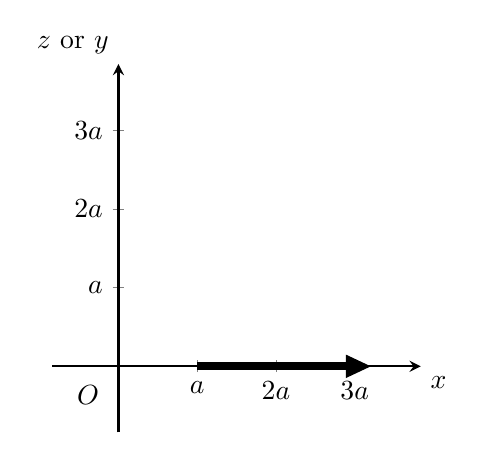
\begin{tikzpicture}
    \begin{axis}[standard,
            xtick={1,2,3},
            ytick={1,2,3},
            samples=1000,
            xlabel={$x$},
            ylabel={$z$ or $y$},
            xmin=-.3,xmax=3.3,
            ymin=-.3,ymax=3.3,
            x=1cm,
            y=1cm/1,
            xticklabels={$a$, $2a$, $3a$},
            yticklabels={$a$, $2a$, $3a$}
           ]
\node[anchor=center,label=south west:$O$] at (axis cs:0,0){};
\draw [line width=1mm](1,0) -- (3,0) node[
    currarrow,
    pos=1, 
    xscale=1,
    sloped,
    scale=1] {};
    \end{axis}
    \end{tikzpicture}
}
\end{center}
\phantomsection
\addcontentsline{toc}{subsubsection}{Region \& Bounds}\textbf{Region \& Bounds}

Our region $R$ will be the quarter circle on the $xy$-plane with radius $a$. Graphically, this looks like
\begin{center}
\resizebox{3.5cm}{!}{
    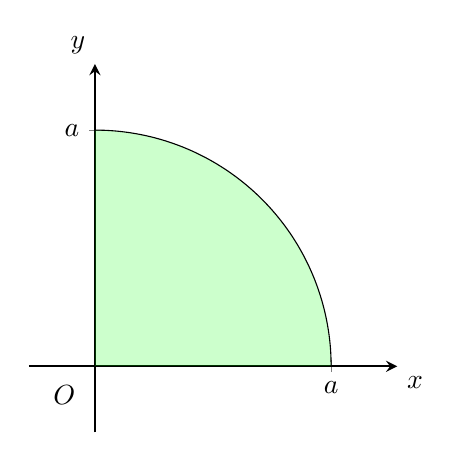
\begin{tikzpicture}
    \begin{axis}[standard,
            xtick={3},
            ytick={3},
            samples=1000,
            xlabel={$x$},
            ylabel={$y$},
            xmin=-.3,xmax=3.3,
            ymin=-.3,ymax=3.3,
            x=1cm,
            y=1cm/1,
            xticklabels={$a$},
            yticklabels={$a$}
           ]
\node[anchor=center,label=south west:$O$] at (axis cs:0,0){};
\addplot[name path=F,domain={0:3}]{sqrt(9-x^2)};
\addplot[name path=G,domain={0:3}]{0};
\addplot[fill=green, fill opacity=0.2] fill between [of=F and G, soft clip={domain=0:3}];
    \end{axis}
    \end{tikzpicture}
}
\end{center}
This will be useful later, but in polar, our lower and upper bounds for $r$ are $r=0$ and $r=a$, respectively. Our lower and upper bounds for $\theta$ are $\theta=0$ and $\theta=\dfrac{\pi}{2}$, respectively.

\phantomsection
\addcontentsline{toc}{subsection}{2(a)}\textbf{(a)} $\F(x,y,z)=\lra{0,0,z}$

\Solution

Recall that if $S$ is given implicitly as $g(x,y,z)=c$, then
\begin{align*}
    \iint_S \F\cdot \n \,d\sigma &= \iint_R \pm \frac{\F\cdot \nabla g}{\left|g_z\right|}\,dA
\end{align*}
Since $\F(x,y,z)=\lra{0,0,z}$, $\nabla g = \lra{2x,2y,2z}$, and $g_z=2z$,
\begin{align*}
   \frac{ \F \cdot \nabla g}{\left|g_z\right|}&=\frac{\lra{0,0,z}\cdot \lra{2x,2y,2z}}{\left|2z\right|}\\
   &=\frac{ \lrp{0+0+2z^2}}{2z}\tag{we're in first octant}\\
   &=\frac{2z^2}{2z}\tag{$2z^2\geq 0$}\\
   &=z\\
   &=\sqrt{a^2-(x^2+y^2)}\tag{$x^2+y^2+z^2=a^2\implies z^2=a^2-(x^2+y^2)$}
\end{align*}
Let's evaluate our integral. We'll probably want to switch to polar, so we'll need to throw in our Jacobian $r$.
\begin{align*}
    \iint_S \F\cdot \n \,d\sigma  &=\iint_R \sqrt{a^2 - (x^2+y^2)}\,dy\,dx\\
    &=\int_0^{\pi/2}\int_0^a \lrp{\sqrt{a^2 - r^2}}r\,dr\,d\theta\tag{in polar, $x^2+y^2=r^2$}\\
    &=\int_0^{\pi/2}\lrb{-\frac{1}{3}(a^2-r^2)^{3/2}}_0^a\,d\theta\tag{or do $u$-sub, $u=a^2-r^2$}\\
    &=\int_0^{\pi/2}\frac{1}{3}(a^2-a^2)^{3/2}-\frac{1}{3}(a^2-0^2)^{3/2}\,d\theta\\
    &=\int_0^{\pi/2}\frac{1}{3}(a^2)^{3/2}\,d\theta\\
    &=\int_0^{\pi/2}\frac{1}{3}a^3\,d\theta\\
    &=\lrb{\frac{1}{3}a^3\theta}_0^{\pi/2}\\
    &=\frac{1}{3}a^3\lrp{\frac{\pi}{2}}\\
    &=\boxed{\frac{\pi}{6}a^3}
\end{align*}

\phantomsection
\addcontentsline{toc}{subsection}{2(b)}\textbf{(b)} $\F(x,y,z)=\lra{y,-x,1}$

\Solution

Recall that if $S$ is given implicitly as $g(x,y,z)=c$, then
\begin{align*}
    \iint_S \F\cdot \n \,d\sigma &= \iint_R \pm \frac{\F\cdot \nabla g}{\left|g_z\right|}\,dA
\end{align*}
Since $\F(x,y,z)=\lra{y,-x,1}$, $\nabla g = \lra{2x,2y,2z}$, and $g_z=2z$,
\begin{align*}
    \frac{ \F \cdot \nabla g}{\left|g_z\right|}&=\frac{ \lra{y,-x,1}\cdot \lra{2x,2y,2z}}{\left|2z\right|}\\
    &=\frac{ \lrp{2xy-2xy+2z}}{2z}\tag{we're in the first octant}\\
    &=\frac{2z}{2z}\\
    &=1
\end{align*}
Let's evaluate our integral. We'll probably want to switch to polar, so we'll need to throw in our Jacobian $r$.
\begin{align*}
   \iint_S \F\cdot \n \,d\sigma&= \iint_S 1\,dy\,dx\\
    &=\int_0^{\pi/2}\int_0^a \lrp{1}r\,dr\,d\theta\\
    &=\int_0^{\pi/2}\lrb{\frac{1}{2}r^2}_0^a\,d\theta\\
    &=\int_0^{\pi/2}\frac{1}{2}a^2\,d\theta\\
    &=\lrb{\frac{1}{2}a^2\theta}_0^{\pi/2}\\
    &=\frac{1}{2}a^2\lrp{\frac{\pi}{2}}\\
    &=\boxed{\frac{1}{4}\pi a^2}
\end{align*}

\phantomsection
\addcontentsline{toc}{subsection}{2(c)}\textbf{(c)} $\F(x,y,z)=\lra{zx,zy,z^2}$

\Solution

Recall that if $S$ is given implicitly as $g(x,y,z)=c$, then
\begin{align*}
    \iint_S \F\cdot \n \,d\sigma &= \iint_R \pm \frac{\F\cdot \nabla g}{\left|g_z\right|}\,dA
\end{align*}
Since $\F(x,y,z)=\lra{zx,zy,z^2}$, $\nabla g = \lra{2x,2y,2z}$, and $g_z=2z$,
\begin{align*}
    \frac{ \F \cdot \nabla g}{\left|g_z\right|}&=\frac{ \lra{zx,zy,z^2}\cdot \lra{2x,2y,2z}}{\left|2z\right|}\\
    &=\frac{ \lrp{2x^2z+2y^2z+2z^3}}{2z}\tag{we're in first octant}\\
    &=\frac{2z(x^2+y^2+z^2)}{2z}\\
    &= x^2+y^2+z^2\\
    &=a^2\tag{$x^2+y^2+z^2=a^2$}
\end{align*}
Let's evaluate our integral. We'll probably want to switch to polar, so we'll need to throw in our Jacobian $r$.
\begin{align*}
 \iint_S \F\cdot \n\,d\sigma   &=\iint_R a^2\,dA\\
    &\int_0^{\pi/2}\int_0^a \lrp{a^2}r\,dr\,d\theta\\
    &=\int_0^{\pi/2}\lrb{\frac{1}{2}a^2r^2}_0^a\,d\theta\\
    &=\int_0^{\pi/2}\frac{1}{2}a^4\,d\theta\\
    &=\lrb{\frac{1}{2}a^4\theta}_0^{\pi/2}\\
    &=\frac{1}{2}a^4\lrp{\frac{\pi}{2}}\\
    &=\boxed{\frac{1}{4}\pi a^4}
\end{align*}

\phantomsection
\addcontentsline{toc}{subsection}{2(d)}\textbf{(d)} $\displaystyle \F(x,y,z)=\frac{\lra{x,y,z}}{\sqrt{x^2+y^2+z^2}}$

\Solution

Recall that if $S$ is given implicitly as $g(x,y,z)=c$, then
\begin{align*}
    \iint_S \F\cdot \n \,d\sigma &= \iint_R \pm \frac{\F\cdot \nabla g}{\left|g_z\right|}\,dA
\end{align*}
Since $\displaystyle \F(x,y,z)=\frac{\lra{x,y,z}}{\sqrt{x^2+y^2+z^2}}$, $\nabla g = \lra{2x,2y,2z}$, and $g_z=2z$,
\begin{align*}
     \frac{ \F \cdot \nabla g}{\left|g_z\right|}&=\frac{ \frac{\lra{x,y,z}}{\sqrt{x^2+y^2+z^2}}\cdot \lra{2x,2y,2z}}{\left|2z\right|}\\
     &=\frac{ \lrp{\frac{2x^2+2y^2+2z^2}{\sqrt{x^2+y^2+z^2}}}}{2z}\tag{we're in the first octant}\\
     &=\frac{ \lrp{\frac{2(x^2+y^2+z^2)}{\sqrt{x^2+y^2+z^2}}}}{2z}\\
     &=\frac{\lrp{\frac{2a^2}{\sqrt{a^2}}}}{2z}\tag{$x^2+y^2+z^2=a^2$}\\
     &=\frac{ \frac{2a^2}{a}}{2z}\\
     &=\frac{ 2a}{2z}\\
     &=\frac{a}{z}\\
     &=\frac{a}{\sqrt{a^2-(x^2+y^2)}}\tag{$x^2+y^2+z^2=a^2\implies z^2 = a^2-(x^2+y^2)$}
\end{align*}
Let's evaluate our integral. We'll probably want to switch to polar, so we'll need to throw in our Jacobian $r$.
\begin{align*}
    \iint_S \F\cdot\n\,d\sigma &=\iint_R \frac{a}{\sqrt{a^2-(x^2+y^2)}}\,dA\\
    &=\int_0^{\pi/2}\int_0^a \lrp{\frac{a}{\sqrt{a^2 - r^2}}}r\,dr\,d\theta\tag{in polar, $x^2+y^2=r^2$}\\
    &u=a^2-r^2\hspace{2em}du=-2r\,dr\\
    &u(0)=a^2\hspace{2em}u(a)=0\\
    &=\int_0^{\pi/2}\int_{a^2}^0 -\frac{a}{2\sqrt{u}}\,du\,d\theta\\
    &=\int_0^{\pi/2}\int_0^{a^2}\frac{a}{2}u^{-1/2}\,du\,d\theta\tag{we gotta flip the bounds}\\
    &=\int_0^{\pi/2}\lrb{au^{1/2}}_0^{a^2}\,d\theta\\
    &=\int_0^{\pi/2} a(a^2)^{1/2}\,d\theta\\
    &=\int_0^{\pi/2}a(a)\,d\theta\\
    &=\int_0^{\pi/2}a^2\,d\theta\\
    &=\lrb{a^2\theta}_0^{\pi/2}\\
    &=a^2\lrp{\frac{\pi}{2}}\\
    &=\boxed{\frac{1}{2}\pi a^2}
\end{align*}

\phantomsection
\addcontentsline{toc}{section}{Problem 3}\textbf{Problem 3}

Find the flux of the field $\F(x,y,z)=\lra{4x,4y,2}$ outward (away from the $z$-axis) through the surface cut from the bottom of the paraboloid $z=x^2+y^2$ by the plane $z=1$.

\Solution

The $x^2+y^2$ makes me think we should parameterize our surface using cylindrical coordinates ($x=r\cos\theta$, $y=r\sin\theta$, $z=z$). Since $z=x^2+y^2$, in cylindrical coordinates, $z=r^2$.  Let $\r(r,\theta)=\lra{r\cos\theta, r\sin\theta, r^2}$.

Let's find the bounds for $r$ and $\theta$.

For $r$,

We can get the lower and upper bounds for $r$ from $0\leq z\leq 1$.
\begin{align*}
    0\leq & z\leq 1\\
    0 \leq & r^2 \leq 1\tag{$z=r^2$}\\
    0 \leq & r\leq 1\tag{$r\geq 0$ always}
\end{align*}
Therefore our lower and upper bounds for $r$ are $r=0$ and $r=1$, respectively.

For $\theta$, 

Since we're going around the entire paraboloid, $0\leq \theta\leq 2\pi$.

Therefore our parameterization (bounds included) is $\r(r,\theta)=\lra{r\cos\theta, r\sin\theta, r^2}$ where $0\leq r\leq 1$ and $0\leq \theta\leq 2\pi$.

Recall that if $S$ is given by the parameterization $\r(u,v)=\lra{x,y,z}$, then
\begin{align*}
    \text{flux}=\iint_S \F\cdot \n \,d\sigma &= \iint_R \F \cdot \lrp{\frac{\partial \r}{\partial u}\times \frac{\partial \r}{\partial v}}\,dA
\end{align*}
In this problem, let's have our $u$ be $r$ and our $v$ be $\theta$.

Since $\r(r,\theta)=\lra{r\cos\theta, r\sin\theta, r^2}$,
\begin{align*}
    \F &= \lra{4r\cos\theta, 4r\sin\theta, 2}\\
    \frac{\partial \r}{\partial r}&-\lra{\cos\theta, \sin\theta, 2r}\\
    \frac{\partial \r}{\partial \theta}&=\lra{-r\sin\theta, r\cos\theta, 0}\\
     \frac{\partial \r}{\partial r}\times \frac{\partial \r}{\partial \theta}&=\begin{vmatrix}\i & \j & \k\\
     \cos \theta & \sin\theta & 2r\\
     -r\sin\theta & r\cos\theta & 0\end{vmatrix}\\
     &=\lrp{0-2r^2\cos\theta}-\lrp{0+2r^2\sin\theta}\j +\lrp{r\cos^2\theta+r\sin^2\theta}\k\\
     &=\lrp{-2r^2\cos\theta}-\lrp{2r^2\sin\theta}\j +\big(r\lrp{\cos^2\theta+\sin^2\theta}\big)\k\\
     &=\lrp{-2r^2\cos\theta}-\lrp{2r^2\sin\theta}\j+\lrp{r}\k\tag{$\cos^2\theta+\sin^2\theta=1$}\\
     &=\lra{-2r^2\cos\theta,-2r^2\sin\theta, r}
     \end{align*}
Let's check if $\displaystyle \frac{\partial \r}{\partial r}\times  \frac{\partial \r }{\partial \theta}=\lra{-2r^2\cos\theta,-2r^2\sin\theta, r}$ is in the right direction.

For no particular reason, at $r=1$ and $\theta =0$, we get the point $(1,0,1)$ from our parameterization $\r(r,\theta)=\lra{r\cos\theta, r\sin\theta, r^2}$. When $r=1$ and $\theta=0$, $\displaystyle \frac{\partial \r}{\partial r}\times  \frac{\partial \r }{\partial \theta}=\lra{-2,0,1}$ which is pointing toward the $z$-axis. Since $\lra{-2,0,1}$ at $(1,0,1)$ points toward the $z$-axis, our direction for $\displaystyle \frac{\partial \r}{\partial r}\times  \frac{\partial \r }{\partial \theta}$ needs to be reversed to become $\displaystyle \frac{\partial \r}{\partial r}\times  \frac{\partial \r }{\partial \theta}=\lra{2r\cos\theta, 2r\sin\theta, -r}$.
\begin{center}
\resizebox{5cm}{!}{
    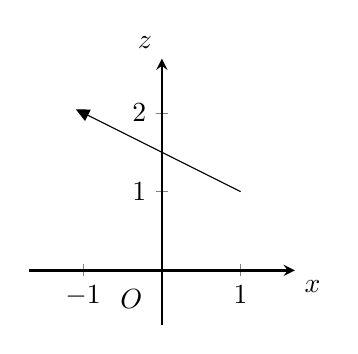
\begin{tikzpicture}
    \begin{axis}[standard,
            xtick={-1,1},
            ytick={1,2},
            samples=1000,
            xlabel={$x$},
            ylabel={$z$},
            xmin=-1.3,xmax=1.3,
            ymin=-.3,ymax=2.3,
            x=1cm,
            y=1cm/1,
           ]
\node[anchor=center,label=south west:$O$] at (axis cs:0,0){};
\draw (1,1) -- (-1,2) node[
    currarrow,
    pos=1, 
    xscale=-1,
    sloped,
    scale=1] {};
    \end{axis}
    \end{tikzpicture}
}
\end{center}
Since $\displaystyle \frac{\partial \r}{\partial r}\times  \frac{\partial \r }{\partial \theta}=\lra{2r\cos\theta, 2r\sin\theta, -r}$,
     \begin{align*}
     \F\cdot \lrp{ \frac{\partial \r}{\partial r}\times \frac{\partial \r}{\partial \theta}}&=\lra{4r\cos\theta, 4r\sin\theta, 2}\cdot\lra{2r^2\cos\theta,2r^2\sin\theta, -r}\\
     &=8r^3\cos^2\theta+ 8r^3\sin^2 \theta-2r\\
     &=8r^3\lrp{\cos^2\theta+\sin^2\theta}-2r\\
     &=8r^3-2r\tag{$\cos^2\theta+\sin^2\theta=1$}
\end{align*}
Let's evaluate our integral.
\begin{align*}
   \text{flux} &=\int_0^{2\pi}\int_0^1 8r^3-2r\,dr\,d\theta\\
    &=\int_0^{2\pi}\lrb{2r^4-r^2}_0^1\,d\theta\\
    &=\int_0^{2\pi} 2 - 1\,d\theta\\
    &=\int_0^{2\pi} 1\,d\theta\\
    &=\lrb{\theta}_0^{2\pi}\\
    &=\boxed{2\pi}
\end{align*}

\newpage
\phantomsection
\addcontentsline{toc}{section}{Problem 4}\textbf{Problem 4}

Let $S$ be the portion of the cylinder $y=\ln x$ in the first octant whose projection onto the $xz$-plane is the rectangle $1\leq x\leq e$, $0\leq z\leq 1$. Find the flux of $\F(x,y,z)=\lra{0,2y,z}$ through $S$ in the direction away from the $xz$-plane.

\Solution

Let's do an implicit method because cross products are no fun. The explict method is fine too. You would just have $\r(x,z)=\lra{x,\ln x, z}$ where $1\leq x\leq e$ and $0\leq z \leq 1$.

Recall that if $S$ is given implicitly as $g(x,y,z)=c$, then
\begin{align*}
   \text{flux}= \iint_S \F\cdot \n \,d\sigma &= \iint_R \pm \frac{\F\cdot \nabla g}{\left|g_y\right|}\,dA
\end{align*}
Let $g(x,y,z)=-\ln x + y = 0$ where $y$ is a function implicitly defined by $x$ and $z$. Then,
\begin{align*}
    \nabla g &= \lra{-\frac{1}{x}, 1,0}\\
    g_y&=1
\end{align*}
Let's check if $\nabla g =\lra{-\dfrac{1}{x},1,0}$ is in the right direction.

For no particular reason, at $x=1$, $y=0$, and $z=0$, we get the point $(1,0,0)$. When $x=1$, $y=0$, and $z=0$, $\nabla g =\lra{-1, 1,0}$. Since $\lra{-1,1,0}$ at $(1,0,0)$ points away from the $xz$-plane, our direction for $\nabla g$ is correct.
\begin{center}
\resizebox{6cm}{!}{
    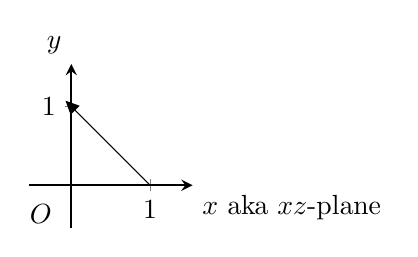
\begin{tikzpicture}
    \begin{axis}[standard,
            xtick={1},
            ytick={1},
            samples=1000,
            xlabel={$x$ aka $xz$-plane},
            ylabel={$y$},
            xmin=-.3,xmax=1.3,
            ymin=-.3,ymax=1.3,
            x=1cm,
            y=1cm/1,
           ]
\node[anchor=center,label=south west:$O$] at (axis cs:0,0){};
\draw (1,0) -- (0,1) node[
    currarrow,
    pos=1, 
    xscale=-1,
    sloped,
    scale=1] {};
    \end{axis}
    \end{tikzpicture}
}
\end{center}
Since $\nabla g =\lra{-\dfrac{1}{x},1,0}$,
\begin{align*}
   \frac{ \F\cdot \nabla g}{\left|g_y\right|}&=\frac{\lra{0,2y,z}\cdot \lra{-\frac{1}{x},1,0}}{\left| 1\right|}\\
   &=\frac{ (0 + 2y+0)}{1}\\
   &=2y\\
   &=2\ln x\tag{$y=\ln x$}
\end{align*}
Let's evaluate our integral.
\begin{align*}
    \text{flux}&=\int_1^e\int_0^1 2 \ln x \,dz\,dx\\
    &=\int_1^e \lrb{(2\ln x) z}_0^1 \,dx\\
    &=\int_1^e 2\ln x\,dx\\
    &u=\ln x \hspace{2em}dv = 2\,dx\\
    &du=\frac{1}{x}\,dx\hspace{2em}v=2x\\
    &=\lrb{2x\ln x}_1^e - \int_1^e 2x\lrp{\frac{1}{x}\,dx}\\
    &=\lrp{2e\ln e - 2\ln 1}-\int_1^e 2\,dx\\
&=\lrp{2e - 0}-\lrb{2x}_1^e\\
&=\lrp{2e}-\lrp{2e- 2}\\
&=2x-2e+2\\
    &=\boxed{2}
\end{align*}
\end{document}